\documentclass[11pt,a4paper]{article}
\usepackage[margin=2.0cm]{geometry}
\usepackage{booktabs}
\usepackage{graphicx}
\usepackage{xcolor}
\usepackage{hyperref}
\hypersetup{colorlinks=true,linkcolor=blue!60!black,urlcolor=blue!60!black}

\title{pypresso on a GPU against Quantum ESPRESSO\\[3pt]
\large twelve cases across the physics, one H200 against one CPU core}
\author{generated by \texttt{performance/plot\_gpu\_sweep.py} from \texttt{gpu-sweep.json}}
\date{2026-08-26}

\begin{document}
\maketitle

\section*{Read the baseline before the ratio}

\textbf{This is the comparison \texttt{GPU.md} \S2.3 rules out by default}, and the
reason is not pedantry. The project's standing metric is single-core pypresso
against single-core Quantum ESPRESSO, so that a ratio measures \emph{code}. A GPU
number against a serial CPU number measures code \emph{and} hardware at once and
cannot be decomposed afterwards. It is reported here because it was asked for,
with the baseline named in every row.

Two further things bound how far these numbers travel:

\begin{itemize}
  \item \textbf{One core is the softest baseline available.} For a single
    $k$-point \texttt{pw.x} has only plane-wave parallelism and saturates early
    --- measured elsewhere in \texttt{PERFORMANCE.md}, 16 to 32 cores buys 4\%,
    and against 32 cores the same silicon comparison falls to about 1x.
  \item \textbf{The iteration counts differ, in both directions.} pypresso takes
    fewer iterations than QE on silicon and five times as many on
    \texttt{ni10-ldau}. That is mixing and starting guess, not hardware, and it
    would show identically on a CPU. \emph{The per-iteration column is the code
    comparison; the total column is time-to-answer.}
\end{itemize}

\begin{center}
\begin{tabular}{ll}
\toprule
GPU & NVIDIA H200 (141 GB) \\
CPU baseline & AMD EPYC / Intel Xeon Cascade Lake, 1 core \\
reference code & Quantum ESPRESSO 7.2 (serial, 1 MPI task) \\
pypresso & commit \texttt{c5dc7d4}, JAX 0.11.1 + jax-cuda12-plugin 0.11.1 \\
settings & pypresso: k\_batch=all, band\_batch=all, \texttt{conv\_thr} = 1e-10 \\
date & 2026-08-26 \\
\bottomrule
\end{tabular}
\end{center}

\begin{figure}[htbp]
\centering
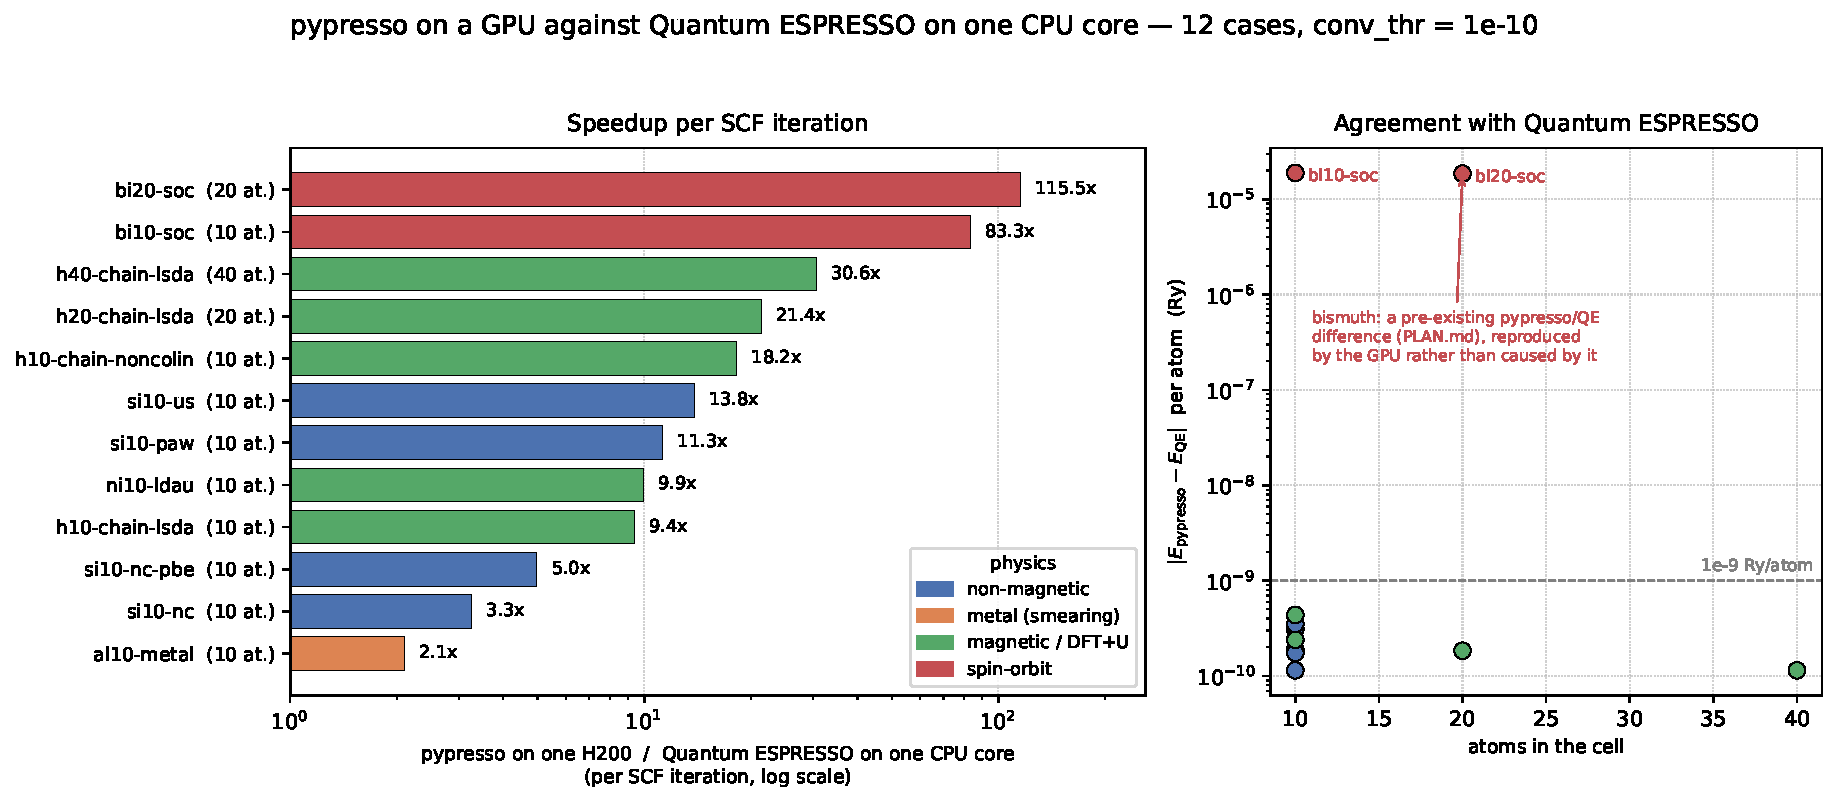
\includegraphics[width=\textwidth]{gpu-sweep-fig.pdf}
\caption{\textbf{Left:} speedup per SCF iteration, sorted, on a log axis because
it spans two decades. \textbf{Right:} the agreement the timings rest on. The
colour is the physics in both panels.}
\label{fig:sweep}
\end{figure}

\section*{What it costs}

\begin{table}[htbp]
\centering
\small
\begin{tabular}{llrrrrrrrr}
\toprule
 & & & & \multicolumn{2}{c}{QE, 1 core} & \multicolumn{2}{c}{pypresso, H200}
 & \multicolumn{2}{c}{speedup} \\
\cmidrule(lr){5-6}\cmidrule(lr){7-8}\cmidrule(lr){9-10}
case & physics & at. & $k$ & it. & ms/it & it. & ms/it & per it. & total \\
\midrule
\texttt{si10-nc} & norm-conserving & 10 & 7 & 14 & 98 & 8 & 30 & \textbf{3.3x} & 5.7x \\
\texttt{si10-nc-pbe} & GGA (PBE) & 10 & 7 & 16 & 221 & 8 & 44 & \textbf{5.0x} & 10.0x \\
\texttt{si10-paw} & PAW & 10 & 7 & 14 & 644 & 8 & 57 & \textbf{11.3x} & 19.7x \\
\texttt{si10-us} & ultrasoft & 10 & 7 & 15 & 595 & 8 & 43 & \textbf{13.8x} & 26.0x \\
\texttt{al10-metal} & metal, smearing & 10 & 10 & 47 & 266 & 10 & 127 & \textbf{2.1x} & 9.9x \\
\texttt{h10-chain-lsda} & collinear magnetic & 10 & 2 & 12 & 1219 & 17 & 130 & \textbf{9.4x} & 6.6x \\
\texttt{h10-chain-noncolin} & noncollinear & 10 & 2 & 13 & 2942 & 17 & 161 & \textbf{18.2x} & 14.0x \\
\texttt{ni10-ldau} & DFT+U, magnetic & 10 & 10 & 29 & 3191 & 151 & 321 & \textbf{9.9x} & 1.9x \\
\texttt{h20-chain-lsda} & collinear magnetic & 20 & 1 & 15 & 2991 & 33 & 140 & \textbf{21.4x} & 9.7x \\
\texttt{h40-chain-lsda} & collinear magnetic & 40 & 1 & 22 & 12669 & 104 & 414 & \textbf{30.6x} & 6.5x \\
\texttt{bi10-soc} & spin-orbit & 10 & 1 & 14 & 21686 & 17 & 260 & \textbf{83.3x} & 68.6x \\
\texttt{bi20-soc} & spin-orbit & 20 & 1 & 20 & 105350 & 20 & 912 & \textbf{115.5x} & 115.5x \\
\bottomrule
\end{tabular}
\caption{Every case converged to \texttt{conv\_thr} = 1e-10. QE's times are its
own timing report (\texttt{electrons}), not a stopwatch around the process;
pypresso's are the warm SCF, with compilation reported separately and never
amortised into the loop.}
\label{tab:timing}
\end{table}

\textbf{The speedup is not one number, and what it tracks is work per $k$-point.}
It runs from 2.1x on \texttt{al10-metal} --- a cheap cell where a single core is
already efficient and the GPU is mostly idle --- to 115.5x on \texttt{bi20-soc},
where QE spends 105\,s \emph{per iteration} on two-component spinors with a
fully-relativistic ultrasoft dataset and the GPU spends 0.91\,s. The
ordering in Figure~\ref{fig:sweep} is the physics: norm-conserving and metallic
cells at the bottom, ultrasoft, PAW and magnetism in the middle, spin-orbit at
the top.

\section*{Whether it is right}

\begin{table}[htbp]
\centering
\small
\begin{tabular}{lrrrrr}
\toprule
case & at. & QE total energy (Ry) & pypresso (Ry) & $\Delta E$ (Ry) & peak GPU (GB) \\
\midrule
\texttt{si10-nc} & 10 & -78.99748976 & -78.99748976 & -3.1e-09 & 0.18 \\
\texttt{si10-nc-pbe} & 10 & -78.65632709 & -78.65632709 & -1.7e-09 & 0.39 \\
\texttt{si10-paw} & 10 & -446.39712348 & -446.39712348 & -3.5e-09 & 0.66 \\
\texttt{si10-us} & 10 & -113.78984345 & -113.78984345 & -1.1e-09 & 0.65 \\
\texttt{al10-metal} & 10 & -41.85395892 & -41.85395892 & -1.9e-09 & 0.40 \\
\texttt{h10-chain-lsda} & 10 & -9.56782281 & -9.56782281 & -4.3e-09 & 0.55 \\
\texttt{h10-chain-noncolin} & 10 & -9.56782281 & -9.56782281 & -4.4e-09 & 1.37 \\
\texttt{ni10-ldau} & 10 & -856.58261082 & -856.58261082 & +2.4e-09 & 1.60 \\
\texttt{h20-chain-lsda} & 20 & -19.13564562 & -19.13564562 & +3.7e-09 & 1.10 \\
\texttt{h40-chain-lsda} & 40 & -38.27138667 & -38.27138667 & +4.6e-09 & 4.06 \\
\texttt{bi10-soc} & 10 & -1477.73706506 & -1477.73725394 & -1.9e-04 $^\dagger$ & 16.92 \\
\texttt{bi20-soc} & 20 & -2955.16301232 & -2955.16338417 & -3.7e-04 $^\dagger$ & 34.70 \\
\bottomrule
\end{tabular}
\caption{$^\dagger$ The bismuth rows are a \emph{pre-existing} pypresso/QE
difference, recorded in \texttt{PLAN.md} as ``the one that does not close'' at
1.9e-4\,Ry, not something the GPU introduces --- and QE 7.5 and 7.2 agree with
each other to 1e-8 on that case, so it is not a version effect either.}
\label{tab:energy}
\end{table}

Every case that does not involve spin-orbit agrees with Quantum ESPRESSO to
4.6e-09\,Ry or better, and those figures reproduce the \emph{CPU} agreements
already recorded in \texttt{PLAN.md} --- 1.9e-9 on \texttt{al10-metal}, 4.3e-9 on
\texttt{h10-chain-lsda}, 4.4e-9 on \texttt{h10-chain-noncolin}. \textbf{The GPU
reproduces pypresso's behaviour, including its known imperfections, rather than
having a numerical character of its own.}

\section*{Two things worth carrying}

\textbf{Memory is the constraint that bites, and spin-orbit is where it bites.}
\texttt{bi20-soc} peaked at 34.7\,GB: two-component spinors on a
fully-relativistic ultrasoft dataset. It fits a 141\,GB H200 with room to spare
and \emph{would not fit a 32\,GB V100}, which is the sort of fact that decides
whether a calculation exists rather than how fast it is.

\textbf{An iteration cap is not a convergence failure.} The first run of this
sweep reported \texttt{ni10-ldau} and \texttt{h40-chain-lsda} as not converging
on the GPU. They were hitting \texttt{run\_scf}'s default of 100 iterations,
where the regression suite has always used 200 for exactly those cases;
\texttt{ni10-ldau} reproduces the same non-convergence on a CPU at 100, which is
what settled it. Both converge here, at 151 and 104 iterations.

\end{document}
